\documentclass[psfig,11pt]{article} 
 
\textheight 24.4cm
\textwidth 16.59cm
\topmargin -0.0cm
\oddsidemargin -0.04in
\evensidemargin -0.04in
%\usepackage{ams}

\def\normalstretch{1.0}
\def\talllinestretch{1.5}
\def\shortlinestretch{0.8}
\renewcommand{\baselinestretch}{\normalstretch}
\parskip 1ex
\renewcommand{\topfraction}{.75}
\renewcommand{\textfraction}{.20}
\renewcommand{\floatsep}{0.0pt}
\renewcommand{\textfloatsep}{1.0cm}
\renewcommand{\floatpagefraction}{.85}

\def\portindent{\hspace{\parindent}}
\newcommand{\REM}[1]{} 
%\newcommand{\sol}[1]{\noindent\textcolor{red}{{#1}}}
%\newcommand{\solspace}[1]{}
\newcommand{\sol}[1]{\REM{#1}}
\newcommand{\solspace}[1]{\vspace{#1}}

\newif\ifsol
%\soltrue

\newcommand{\Bsol}{\ifsol \noindent \color{red}}
\newcommand{\Esol}[1]{\color{black} 
\else 
\vspace{{#1}} 
 \fi
 }

\input epsf
\usepackage{epsfig}
\usepackage{subfigure}
\usepackage{fullpage}
\usepackage{multirow}
%\usepackage{multicolumn}
\pagestyle{plain}
\usepackage[usenames]{color}

\begin{document}

\newcounter{quest}
\setcounter{quest}{3}
\newenvironment{question}[1][??]{\noindent{\bf Question  \stepcounter{quest}
\arabic{quest} (\textrm{#1} points): }}



\hspace{2in} \hrulefill \hspace{1in}

\renewcommand{\theenumi}{\alph{enumi}}


\color{black}

\begin{figure*}[t]
\begin{center}$
\begin{array}{cc}
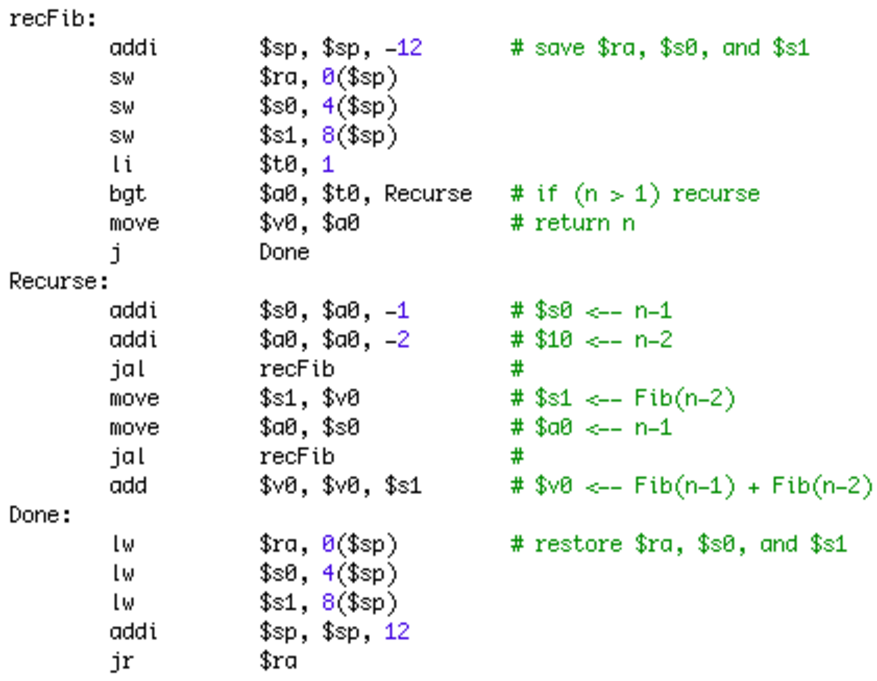
\includegraphics[width=3.5in]{recFib.pdf} &
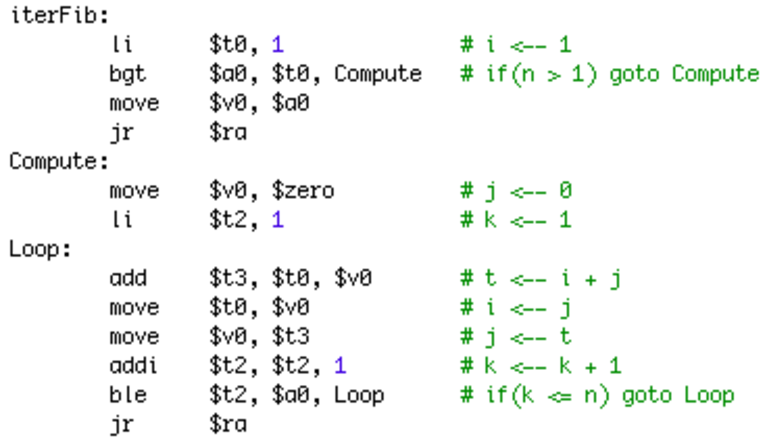
\includegraphics[width=3.0in]{iterFib.pdf} \\
\end{array}$
\caption{\label{fig:Fib} (a) Recursive Fibonacci; (b) Iterative Fibonacci}
\end{center}
\end{figure*}
\begin{question}[20] The Fibonacci sequence is defined as follows:
\begin{eqnarray}
\mathrm{Fib}(n) &=& \left\{
\begin{array}{cl}
\mathrm{Fib}(n-1) + \mathrm{Fib}(n-2) & \mathrm{if } n > 1,\\ \nonumber
n & \mathrm{if } n \leq 1. \nonumber
\end{array} \right. \nonumber
\end{eqnarray}
Figure~\ref{fig:Fib} shows two versions of MIPS assembly program that compute the Fibonacci value of a number $n$, which is the input parameter in {\tt \$a0}.
\begin{enumerate}
\item({\bf 10 points}) Which version, {\tt recFib} or {\tt iterFib}, is more efficient for a large value of $n$? Explain your answer.

\ifsol
\color{red}
The iterative version is more efficient for two reasons.
\begin{enumerate}
\item It does not need to create a stack frame for the multiple calls of the function, and thus is not required to perform expensive memory (load and store) operations.
\item It does not repeat the computation of the Fibonacci of lower values. For instance, to compute the Fibonacci value of $n$ the recursive function calls itself twice: one time with parameter $n-1$ and another with parameter $n-2$. But the computation of $n-1$ will itself call {\tt recFib} with $n-2$, even though it had already been computed.
\end{enumerate}
\color{black}
\else
  \vspace{1.5in}
\fi

\item({\bf 10 points}) Give an expression, in terms of $n$, for the amount of storage, given in bytes, that must be available to grow the stack for each of the subroutines to execute correctly.

\ifsol
\color{red}
\begin{figure*}[t]
\begin{center}$
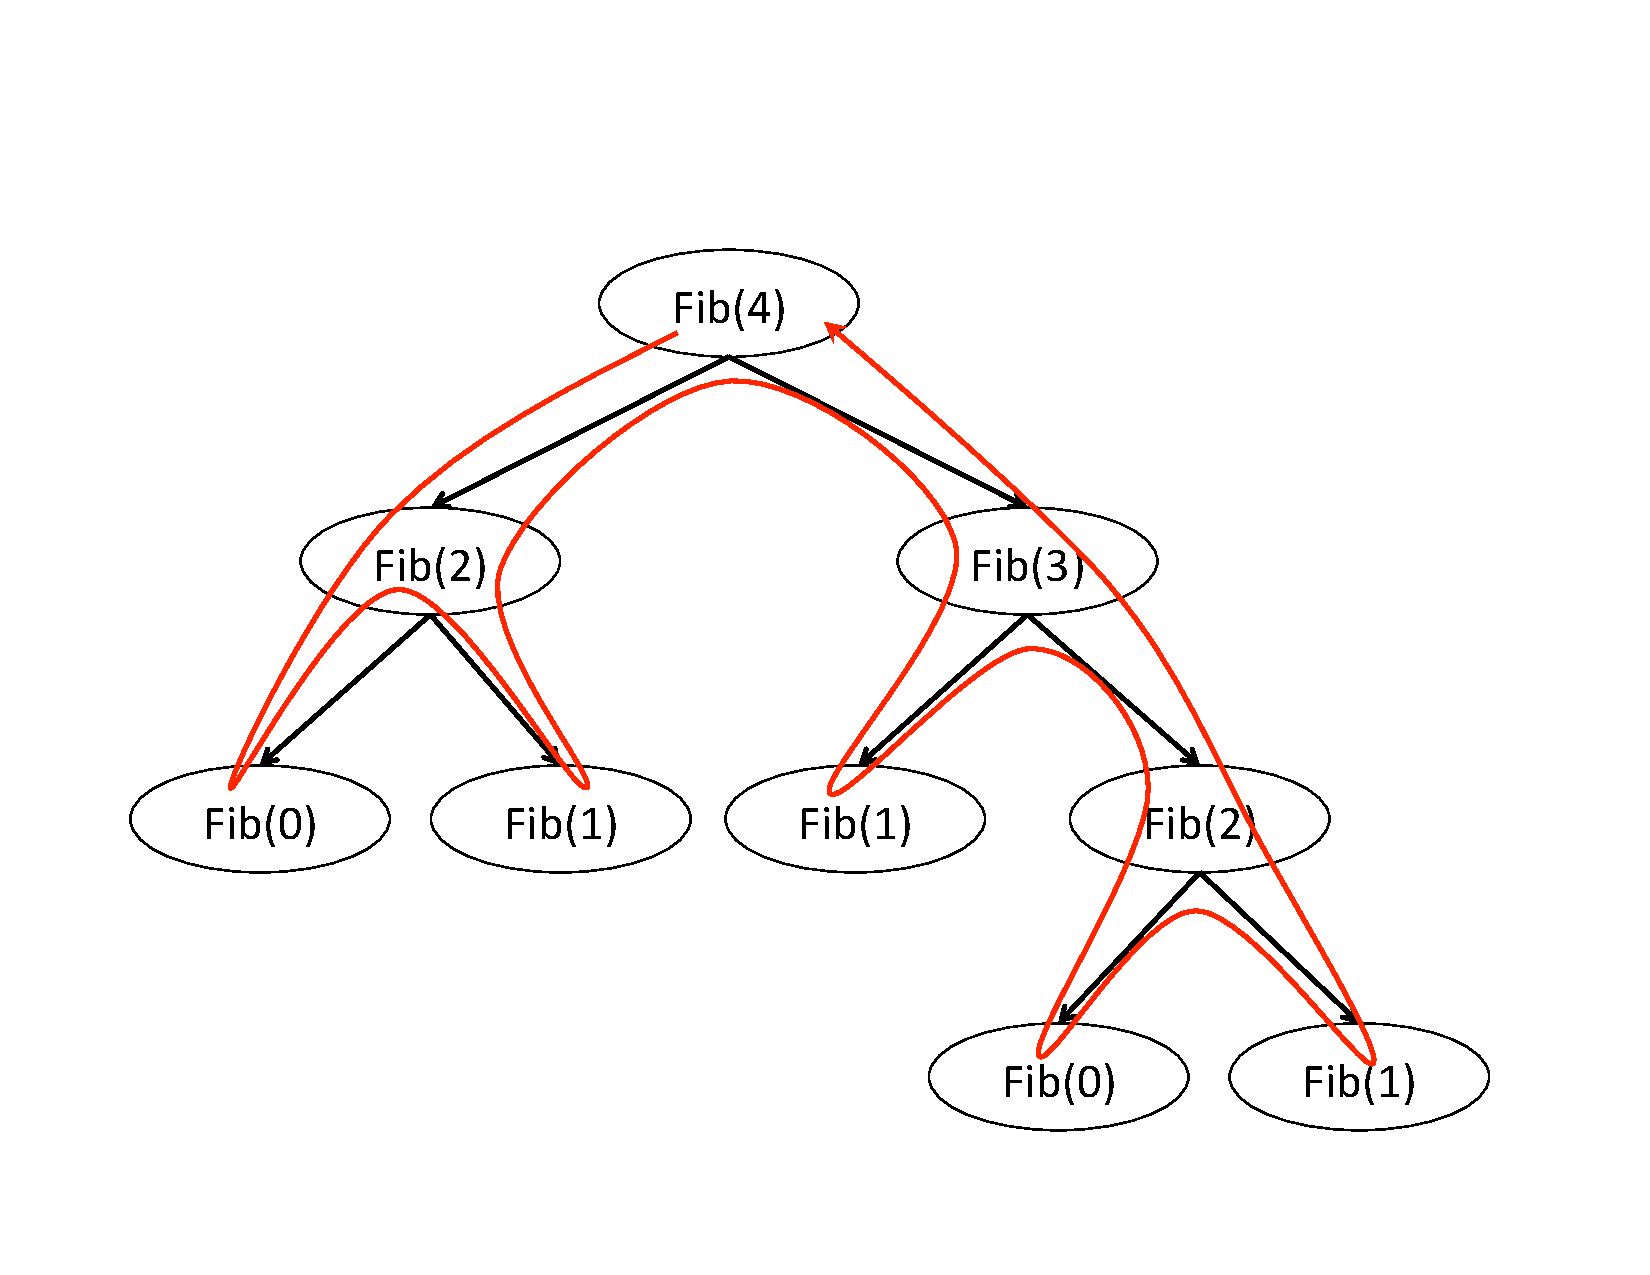
\includegraphics[width=3.5in]{FibRecursion.pdf} 
$
\caption{\label{fig:recFib} (a) Example of recursion in {\tt recFib}}
\end{center}
\end{figure*}
The depth of the stack required grows by 12 bytes every time a recursive call is make and shrinks by 12 bytes every time a recursive call returns. Even though there are two recursive calls for each invocation of {\tt recFib}, they execute sequentially as illustrated in Figure~\ref{fig:recFib}. Thus the space required for the stack, expressed in bytes, is $12 \times n$.
\color{black}
\else
  \vspace{1.5in}
\fi
\end{enumerate}


\end{question}

\end{document}

